\documentclass[12pt,fleqn]{examtst}
\usepackage{graphicx}
\usepackage{amssymb}
\usepackage{amsmath}
\usepackage{listings}
\usepackage{multirow}
\usepackage{multicol}
\usepackage{hhline}
\usepackage{booktabs}
\usepackage{url}
\usepackage{enumerate}
\usepackage{hyperref}
%% Comments

\usepackage{color}

\newif\ifcomments\commentstrue

\ifcomments
\newcommand{\authornote}[3]{\textcolor{#1}{[#3 ---#2]}}
\newcommand{\todo}[1]{\textcolor{red}{[TODO: #1]}}
\else
\newcommand{\authornote}[3]{}
\newcommand{\todo}[1]{}
\fi

\newcommand{\wss}[1]{\authornote{blue}{SS}{#1}}

\begin{document}

\newcommand{\soln}{n} %y for yes and n for no

\lstset{language=python, basicstyle=\ttfamily, breaklines=true,
  showspaces=false, showstringspaces=false, breakatwhitespace=true}

\newcommand{\codeit}[1]{\texttt{\textit{#1}}}

\begin{center}
  {\large \bf COMP SCI 2ME3 and SFWR ENG 2AA4 Midterm Examination}\\[1ex]
  {\large \bf McMaster University}\\[1ex]
  \ifthenelse{\equal{\soln}{y}}{\large {\bf ANSWER KEY} %Large arrow
    %($\Longleftarrow$) for correct% , small ($\leftarrow$) for partially
    % correct
  }{}
\end{center}

\medskip

\noindent
DAY CLASS%, \textbf{Version 1}
\hfill Dr.~S.~Smith \\
DURATION OF EXAMINATION: 3 hours \\
MCMASTER UNIVERSITY MIDTERM EXAMINATION \hfill March 4, 2021

\medskip

\noindent
\rule[3 mm]{\textwidth}{0.5mm}

%\begin{minipage}[t]{1.0\textwidth}

NAME: \wss{Enter your name here}\\[1ex]

Student ID: \wss{Enter your student number here} \\[2mm]

\noindent
\rule[3 mm]{\textwidth}{0.5mm}

This examination paper includes \noofpages pages and
4 % VARIABILITY
questions. You are responsible for ensuring that your copy of the examination
paper is complete. Bring any discrepancy to the attention
of your instructor.\\

\noindent
\emph{By submitting this work, I certify that the work represents solely my own
independent efforts. I confirm that I am expected to exhibit honesty and use
ethical behaviour in all aspects of the learning process.  I confirm that it is
my responsibility to understand what constitutes academic dishonesty under the
\href{https://secretariat.mcmaster.ca/app/uploads/Academic-Integrity-Policy-1-1.pdf}
{Academic Integrity Policy}}.\\

\noindent
\textbf{Special Instructions}:

\begin{enumerate}

\item For taking tests remotely: 
\begin{itemize}
\item Turn off all unnecessary programs, especially Netflix, YouTube, games like
  Xbox or PS4, anything that might be downloading or streaming.
\item If your house is shared, ask others to refrain from doing those activities
  during the test.
\item If you can, connect to the internet via a wired connection.
\item Move close to the Wi-Fi hub in your house. 
\item Restart your computer, 1-2 hours before the exam. A restart can be very
  helpful for several computer hiccups.
\item Commit and push your tex file, compiled pdf file, and code files
  frequently.
\item Ensure that you push your solution (tex file, pdf file and code files)
  before time expires on the test.  The solution that is in the repo at the
  deadline is the solution that will be graded.
\end{itemize}
\item It is your responsibility to ensure that the answer sheet is properly
  completed. Your examination result depends upon proper attention to the
  instructions.
\item All physical external resources are permitted, including textbooks, calculators,
  computers, compilers, and the internet.
\item The work has to be completed individually.  Discussion with others is
  strictly prohibited.
\item Read each question carefully.
\item Try to allocate your time sensibly and divide it appropriately between the
  questions.
\item The set $\mathbb{N}$ is assumed to include $0$.
\end{enumerate}
%\end{minipage}\\

\examheader{CS2ME3/SE2AA4 \ifthenelse{\equal{\soln}{y}} {\hfill SOLUTIONS} }

\renewcommand{\labelenumi}{\Alph{enumi}.}

\newpage

%%%%%%%%%%%%%%%%%%%%%%%%%%%%%%%%%%%%%%%%%%%%%%%%%%%%%%%%%%%%%%%%%%%%%%

\question{6 marks} %tests software qualities - reusability?
Parnas advocates faking a rational design process as depicted in the figure below.
The faked documentation follows these steps: Requirements (SRS) $\rightarrow$
Design (MG and MIS) $\rightarrow$ Application Implementation (code)
$\rightarrow$ Verification and Validation (Unit Testing, Integration Testing,
Review).  How are the principles of
a) abstraction and b) separation of concerns applied in a rational design
process?  In your answer you can refer to any aspects of the process,
documentation, and/or Parnas's principles.

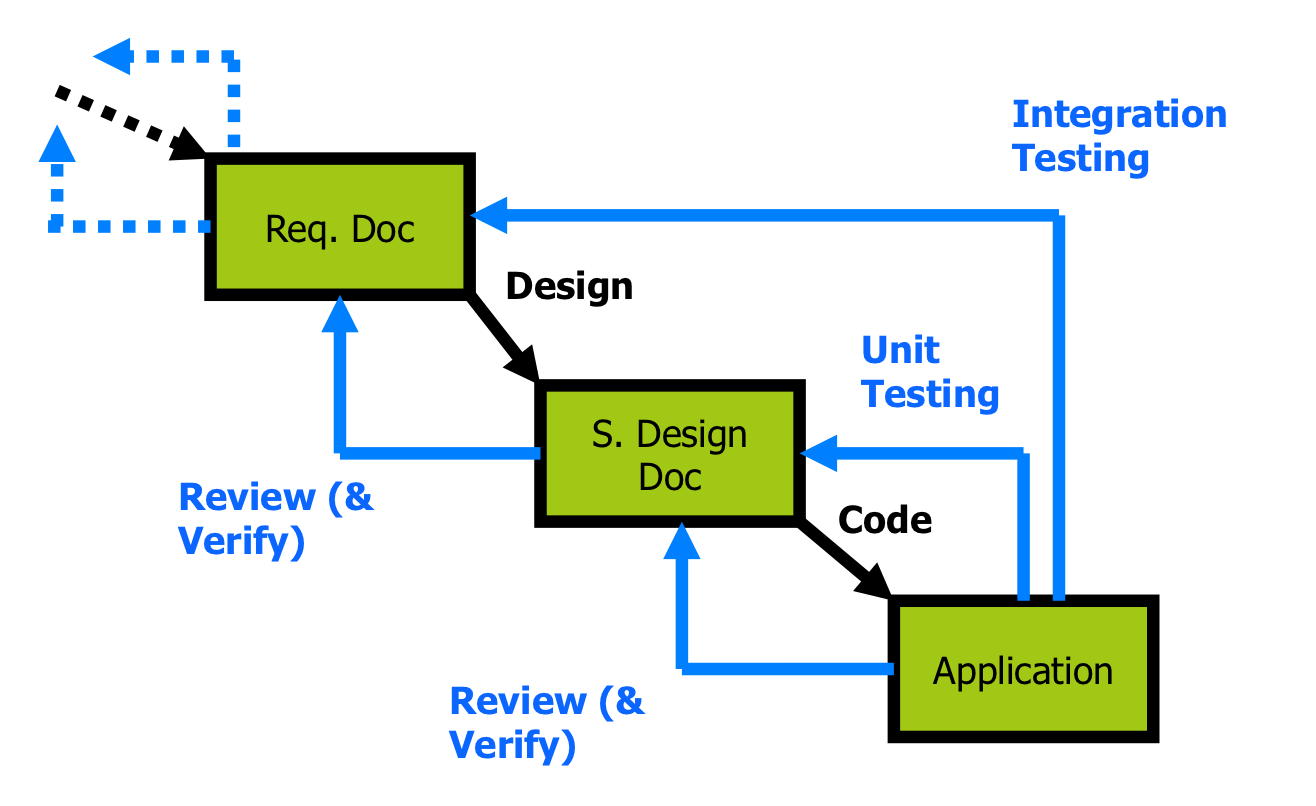
\includegraphics[scale=0.4]{SoftwareLifecycle.png}

\noindent \wss{Fill in your answer below}

\begin{enumerate}[a)]
\item Abstraction
  \begin{itemize}
  \item A rational development process was introduced by Parnas and Clements to provide meaning to the ideal process in which programs are derived from its requirements. Despite claiming that a rational design process is needed in order to produce quality software, it is argued that it is impossible to find a process in which the software is designed in a perfectly rational way. Instead, it is suggested to fake this process, by presenting the system and its associated documents to others as if the user had followed this particular idealized design process. By doing these, any unnecessary details or processes that may have occurred during the authentic design process can be left out for future users. This upholds the concept of abstraction, which is the idea of only focusing on what is important in an implementation, and simply ignoring irrelevant processes and details.
  \item A direct application of the advantages that come with a design that prioritizes abstraction can be described as follows. Once the abstractions of the components public to the user are understood, which in this case would represent the MIS,  all of the components of the design would thus be understood without having to look the internals of the modules. 
  \item This serves useful as there is a common practice in the design process called information hiding, where parts of the module that are likely to change are kept hidden from the user. The purpose of information hiding is to anticipate future changes that could occur with the modules themselves. Therefore, the user is able to implement the design as specified by the given documentation, and have a sought after understanding of only the necessary components without having to have access to the modules that are kept hidden. This directly relates to the hierarchy that is created through the module guide that prioritizes information hiding, as repeated applications of abstraction will essentially produce a hierarchy of models. 

  \end{itemize}
\item Separation of Concerns
  \begin{itemize}
  \item The separation of concerns is a principle that states that every separate concern must be considered separately in order to reduce a complex problem into a set of simpler ones. Parnas’ concept of faking the rational design provides a means of creating this set of simpler problems. 
  \item One way in which this is achieved is through the use of the Module Interface Specification. This specification aims to describe the data and procedures that provide accesses to the services of the modules themselves. An MIS will show what the module does and what services it provides, but it doesn’t tell the user how exactly to implement the modules themselves. This is an effective means of taking the pre-defined problem, and splitting it up so that it can be solved in separate modules that will eventually work together to solve that problem.
  \item Another component of Parnas’ rational design process that follows after the design specification is the Module Guide. The module decomposition must be documented to allow for developers to understand and verify the decomposition itself. There exists a hierarchy that defines the module guide by accomplishing the decomposition of information hidden from the clients, otherwise known as secrets. Through behavioural, software and hardware decision hiding modules that separate the hierarchy into three unique categories, separation of change is infact achieved, and the problem is futher subdivided as one continues down the hierarchy.
  \end{itemize}
\end{enumerate}

%%%%%%%%%%%%%%%%%%%%%%%%%%%%%%%%%%%%%%%%%%%%%%%%%%%%%%%%%%%%%%%%%%%%%%

\newpage

\noindent Consider the specification for two modules: SeqServices and SetOfInt.

\section* {Sequence Services Library}

\subsection*{Module}

SeqServicesLibrary

\subsection* {Uses}

None

\subsection* {Syntax}

\subsubsection* {Exported Constants}

None

\subsubsection* {Exported Types}

None 

\subsubsection* {Exported Access Programs}

\begin{tabular}{| l | l | l | p{5cm} |}
\hline
\textbf{Routine name} & \textbf{In} & \textbf{Out} & \textbf{Exceptions}\\
\hline
max\_val & seq of $\mathbb{Z}$ & $\mathbb{N}$ & ValueError\\
  \hline
count & $\mathbb{Z}$, seq of $\mathbb{Z}$ & $\mathbb{N}$ & ValueError\\
\hline
spices & seq of $\mathbb{Z}$ & seq of string & ValueError\\
\hline
new\_max\_val & seq of $\mathbb{Z}$, $\mathbb{Z} \rightarrow \mathbb{B}$ &
                                                                           $\mathbb{N}$ & ValueError\\
\hline
  
\end{tabular}

\subsection* {Semantics}

\subsubsection* {State Variables}

None

\subsubsection* {State Invariant}

None

\subsubsection* {Assumptions}

\begin{itemize}
\item All access programs will have inputs provided that match the types
  given in the specification.
\end{itemize}

\subsubsection* {Access Routine Semantics}

\noindent max\_val($s$)
\begin{itemize}
\item output: $\mathit{out} := | m |: \mathbb{N} \text{ such that } (m \in s) \wedge
  \forall (x: \mathbb{Z} | x \in s : | m | \geq | x |)$
\item exception: $(|s| = 0 \Rightarrow \text{ValueError})$
\end{itemize}

\noindent count($t, s$)
\begin{itemize}
\item output: $\mathit{out} := + (x: \mathbb{Z} | x \in s \wedge x = t : 1)$
\item exception: $(|s| = 0 \Rightarrow \text{ValueError})$
\end{itemize}

\noindent spices($s$)
\begin{itemize}
\item output: $\mathit{out} := \langle x: \mathbb{Z} | x \in s : (x \leq 0
  \Rightarrow \text{``nutmeg"} | \text{True} \Rightarrow \text{``ginger"}) \rangle$
\item exception: $(|s| = 0 \Rightarrow \text{ValueError})$
\end{itemize}

\noindent new\_max\_val($s$, $f$)
\begin{itemize}
\item output: $\mathit{out} := \text{max\_val}(\langle x: \mathbb{Z} | x \in s
  \wedge f(x): x \rangle )$
\item exception: $(|s| = 0 \Rightarrow \text{ValueError})$
\end{itemize}

%%%%%%%%%%%%%%%%%%%%%%%%%%%%%%%%%%

\newpage

\section* {Set of Integers Abstract Data Type}

\subsection* {Template Module}

SetOfInt

\subsection* {Uses}

None

\subsection* {Syntax}

\subsubsection* {Exported Types}

SetOfInt = ?

\subsubsection* {Exported Constants}

None

\subsubsection* {Exported Access Programs}

\begin{tabular}{| l | l | l | p{6cm} |}
\hline
\textbf{Routine name} & \textbf{In} & \textbf{Out} & \textbf{Exceptions}\\
\hline
new SetOfInt & seq of $\mathbb{Z}$ & SetOfInt & \\
\hline
is\_member & $\mathbb{Z}$ & $\mathbb{B}$ & \\
\hline
to\_seq &  & seq of $\mathbb{Z}$ & \\
\hline
union & SetOfInt & SetOfInt & \\
\hline
diff & SetOfInt & SetOfInt & \\
\hline
size &  & $\mathbb{N}$ & \\
\hline
empty &  & $\mathbb{B}$ & \\
\hline
equals & SetOfInt & $\mathbb{B}$ & \\
\hline

\end{tabular}

\subsection* {Semantics}

\subsubsection* {State Variables}

$s$: set of $\mathbb{Z}$

\subsubsection* {State Invariant}

None

\subsubsection* {Assumptions}

\begin{itemize}
\item The SetOfInt constructor is called for each object instance before any
  other access routine is called for that object.  The constructor can only be
  called once.  All access programs will have inputs provided that match the types
  given in the specification.
\end{itemize}

\subsubsection* {Access Routine Semantics}

\noindent new SetOfInt($x_s$):
\begin{itemize}
\item transition: $s := \cup (x: \mathbb{Z} | x \in x_s : \{ x \} )$
\item output: $\mathit{out} := \mathit{self}$
\item exception: none
\end{itemize}

\noindent is\_member($x$):
\begin{itemize}
\item output: $x \in s$
\item exception: none
\end{itemize}

\noindent to\_seq():
\begin{itemize}
\item output: $out := \mbox{set\_to\_seq}(s)$
\item exception: none
\end{itemize}

\noindent union($t$):
\begin{itemize}
\item output: $\text{SetOfInt} (\mbox{set\_to\_seq}(s) ||
  t.\text{to\_seq()})$

  \textit{\# in case it is clearer, an alternate version of output is:}
  
  $\text{SetOfInt}(\text{set\_to\_seq}(s \cup \{x: \mathbb{Z} | x \in t.\text{to\_seq()} : x \}))$
  
\item exception: none
\end{itemize}

\noindent diff($t$):
\begin{itemize}
\item output:
  $\text{SetOfInt}( \text{set\_to\_seq} (s \cap \text{complement}(t.\text{to\_seq()})))$
  
\item exception: none
\end{itemize}

\noindent size():
\begin{itemize}
\item output: $| s |$
\item exception: none
\end{itemize}

\noindent empty():
\begin{itemize}
\item output: $s = \varnothing$
\item exception: none
\end{itemize}

\noindent equals($t$):
\begin{itemize}
\item output: $\forall ( x: \mathbb{Z} | x \in \mathbb{Z} : x \in
  t.\text{to\_seq()} \leftrightarrow x \in s)$ \textit{\# this means:} $t.\text{to\_seq}() = s$
\item exception: none
\end{itemize}

\subsection*{Local Functions}

\noindent $\mbox{set\_to\_seq}: \text{set of } \mathbb{Z} \rightarrow \mbox{seq of }
\mathbb{Z}$\\
\noindent
$\mbox{set\_to\_seq}(s) \equiv \langle x: \mathbb{Z} | x \in s : x \rangle$
\textit{\# Return a seq of all of the elems in the set s, order does not matter}\\

\noindent $\mbox{complement}: \text{seq of } \mathbb{Z} \rightarrow \mbox{ set of }
\mathbb{Z}$\\
$\mbox{complement}(A) \equiv \{ x: \mathbb{Z} | x \not\in A : x \}$\\

%%%%%%%%%%%%%%%%%%%%%%%%%%%%%%%%%%

\newpage

\noindent
\begin{minipage}{\textwidth}
\question{15 marks} \label{Q_PythonCode}

\wss{Complete Python code to match the above specification.}  The files you need
to complete are: \texttt{SeqServicesLibrary.py} and \texttt{SetOfInt.py}.  Two
testing files are also provided: \texttt{expt.py} and \texttt{test\_driver.py}.
The file \texttt{expt.py} is pre-populated with some simple experiments to help
you see the interface in use, and do some initial test.  You are free to add to
this file to experiment with your work, but the file itself isn't graded.  The
\texttt{test\_driver.py} is also not graded.  However, you may want to create
test cases to improve your confidence in your solution.  The stubs of the
necessary files are already available in your \texttt{src} folder.  The code
will automatically be imported into this document when the \texttt{tex} file is
compiled.  You should use the provided Makefile to test your code.  You will NOT
need to modify the Makefile.  The given Makefile will work for \texttt{make
  test}, without errors, from the initial state of your repo.  The \texttt{make
  expt} rule will also work, because all lines of code have been commented out.
Uncomment lines as you complete work on each part of the modules relevant to
those lines in \texttt{expt.py} file.  The required imports are already given in
the code.  You should not make any modifications in the provided import
statements.  You should not delete the ones that are already there.  Although
you can solve the problem without adding any imports, if your solution requires
additional imports, you can add them.  As usual, the final test is whether the
code runs on mills.

Any exceptions in the specification have names identical to the expected Python
exceptions; your code should use exactly the exception names as given in the
spec.

You do not need to worry about doxygen comments.  However, you should include
regular comments in the code where it would benefit from an explanation.

You do not need to worry about PEP8.  Adherence to PEP8 will not be part of the
grading.

Remember, your code needs to implement the given specification so that the
interface behaves as specified.  This does NOT mean that the local functions
need to all be implemented, or that the types used internally to the spec need
to be implemented exactly as given.  If you do implement any local functions,
please make them private by preceding the name with double underscores.\\

\end{minipage}

\newpage

\subsection*{Code for SeqServicesLibrary.py}

\noindent \lstinputlisting{./src/SeqServicesLibrary.py}

\newpage

\subsection*{Code for SetOfInt.py}

\noindent \lstinputlisting{./src/SetOfInt.py}

\newpage

\subsection*{Code for expt.py}

\noindent \lstinputlisting{./src/expt.py}

\newpage

\subsection*{Code for test\_driver.py}

\noindent \lstinputlisting{./src/test_driver.py}

\newpage

%%%%%%%%%%%%%%%%%%%%%%%%%%%%%%%%%%

\noindent
\begin{minipage}{\textwidth}
\question{5 marks} 

Critique the design of the interface for the SetOfInt module.  Specifically,
review the interface with respect to its consistency, essentiality, generality
and minimality.  Please be specific in your answer.

\wss{Put your answer for each quality below.}

\begin{itemize}
\item \textbf{consistency}: The MIS achieves consistent naming conventions, as there are no instances where the same variable is given different names to potentially confuse the user. Additionally, the ordering of parameters in the argument list is not necessarily an issue because there is only ever a maximum of one input into any of the methods, but this makes the formatting quite clear to the user. In addition, although there are no explicit exceptions mentioned throughout the implementation of the access routine semantics, a clearly defined assumption is stated saying that the types of the input will be correct and that the constructor will be called before any other access routine. A general assumption for the entire module allows for the consistency to be upheld. 
\item \textbf{essentiality}: An MIS should prioritize being essential in order to omit any unnecessary features that may confuse the user or provide them with more than enough information to create a proper implementation. The entire class itself aims to convert sequences to sets and do different operations on these sets, however python’s built-in library has a lot of functionality with such properities through the list() and set() methods. However, the specification itself does do a reasonable job of only including the needed methods and parameters to fully implement the SetOfInt abstract data type. The only exception is the empty() method, that isn’t needed because it’s purpose can be fulfilled through the use of the size() method, as described in the explanation of minimality below.
\item \textbf{generality}: Generality is an important quality to take into consideration as it is not good practice to predict how the module will actually be used. However, because the class only works with integers, this reduces the user’s ability to use the class with sequences of any other type. Therefore, the MIS would not be considered general unless measures were taken within the specification to explicitly state that the sequences can be of any type. 
\item \textbf{minimality}: This MIS does now allow for a minimal implementation of the SetOfInt class due to the fact that it fails to ensure that every access routine is independent. This is because of the implementation of both the size() method and empty() method. It is unnecessary to have a method that checks the size of the set of integers, as well as a method that checks whether or now a set is empty or not. Instead, a way to make this MIS minimal is to eliminate the empty() method all together. If the user wishes to check if the set is empty, they can call on the size() method, where if a value of 0 is returned, then it would indicate that the set is in fact empty.
\end{itemize}

\end{minipage}

%%%%%%%%%%%%%%%%%%%%%%%%%%%%%%%%%%

\newpage

\noindent
\begin{minipage}{\textwidth}
\question{4 marks}

The module SetOfInt is for a set of integers.  Please answer the following
questions related to making that module generic. 
\begin{enumerate}[a.]
\item How would you change the specification to make it generic?  (Specifically
  what changes would you make to the given specification.  You don't need to
  redo the spec, just summarize what changes you would need to make.)
\item What changes would you need to make to the Python
implementation to make it generic for type T?  (Again, you can describe and
characterize the changes; you don't actually have to make them.)
\item What relational operator needs to be defined for type T to be a valid
  choice?
\item BONUS (1 mark) How would you specify (in the MIS) the relational operator
  constraint (from the previous question) on the generic type T?
\end{enumerate}

\wss{Put your answer below.}

\begin{enumerate}[a.]
\item All inputs and outputs will accept either an integer or a sequence of integers according the the design specification. In order to allow for generalization by allowing multiple types, this would be done by generalizing all such inputs and outputs to type T. Specifically, changing all the occurances of $\mathbb{Z}$ to T would make the specification general. Additionally, the name of the module itself can bs changed to Seq, now that it doesn't only work for type integers and sequences of integers. 
\item Making a python implementation generic for type T is useful when the type of data that is wished to be stored is unknown, or if it is desired for the implementation to take on multiple types of data without having to implement extra code for each type. Python achieves this through a method called duck typing, so that it doesn’t need special syntax to handle the multiple types. As long as a variable is not defined to a specific type, for example if x = int(3), then python allows for any type to be used.
\item In order to make type T a valid choice, the equals relation operator needs to be defined for type T. This is because the built in python functionality with equals would not suffice for such sets where the type is not defined.
\item In order to specify this in the MIS, a local function for can be defined that would essentially overwrite the built in python equals method, and instead use the one specified that would work for all types.
\end{enumerate}

\end{minipage}

\end{document}